\documentclass{sig-alternate}
\usepackage{float}
\restylefloat{table}

\title{CSCI-620 Data Management with the IMDb Dataset}
\subtitle{[Understanding, modeling, and developing tools to interact with the IMDb dataset]}
\numberofauthors{4}
\author
{
\alignauthor
  Aishwarya Rao
  \email{ar2711@rit.edu}
\alignauthor
  Apurav Khare
  \email{ak2816@rit.edu}
\and
\alignauthor
  Martin Qian
  \email{jq3513@rit.edu}
\alignauthor
  Prateek Kalasannavar
  \email{pk6685@rit.edu}
}

\begin{document}
\maketitle
\begin{abstract}
This project aims to explore a dataset by understanding it, modeling it to a normalized relational schema so that it can be stored and retrieved from a relational database management system, and building a user-friendly interface to access the data. The end goal of this project is to develop an interface that allows fast and easy access to the dataset with functionalities including search by specific parameters. 
\end{abstract}

\section{The IMDb Dataset}
The dataset chosen for this project is the publicly available IMDb dataset which consists of the title metadata (title here refers to a movie or series), its cast and crew and their metadata, and the ratings for the title. The data is chosen as it publicly available and regularly updated. It is considerably large and requires critical modeling and design to access it efficiently for access through queries.
\subsection{Sample Data}
The IMDb dataset consists of seven zipped files including the title, crew, actor names, and ratings. Each of these files have their own attributes represented in the tab spaced formatting. The challenges offered by this dataset include modeling of the data by keeping in mind both the normalization constraints as well as the current database structure, handling multi-value attributes that are present in some of the tables, and designing a script and model capable of handling missing values for some attributes. Figure \ref{sample} depicts what the data looks like.
\begin{figure}
	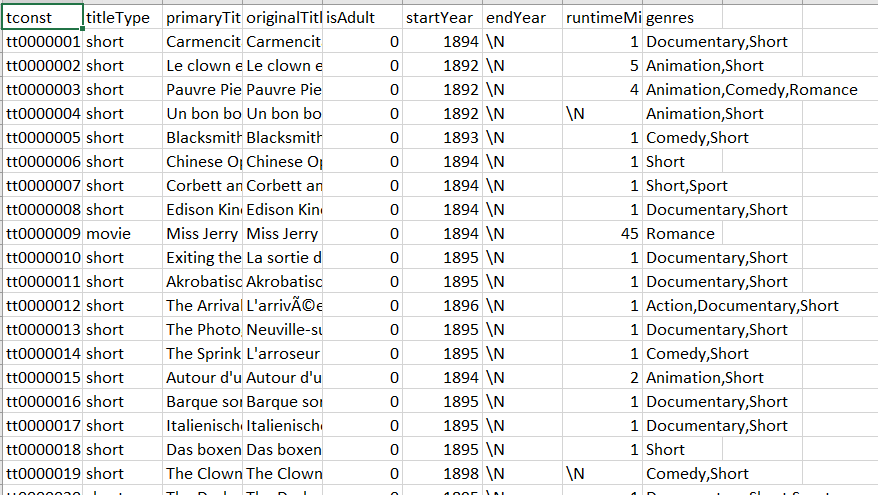
\includegraphics[width = \linewidth]{sample.png}
	\caption{Sample data from table title}
	\label{sample}
\end{figure}
\section{Project Outline}
\subsection{Data Modeling}
In this phase, we understand and explore the data thoroughly to identify entities, their relations with each other, and all relevant constraints. The outcome of this phase will be an ER diagram that summarizes the observations by week 4. 
\subsection{Schema Identification}
This phase involves the identification and mapping of the relational schema from the entity- relationship Model, as well as choose appropriate constraints and keys required to maintain data integrity and avoid redundancies. This phase ends by week 5 with the predicted deliverable as the populated relational database system.
\subsection{Create Queries}
The next phase in the project will involve identifying possible use-case scenarios of the dataset and building equivalent queries to handle these requests. These queries will include searching by title, actor, genre, or other attributes. It will also allow sorting by year, title, or any other appropriate parameter. This phase will also require testing and refining the queries that are built. The deliverable for this phase is the SQL script for database access and is expected to be completed by week 7.
\subsection{User Interface Development}
In this phase, we develop an user-friendly interface for potential customers to interact with the database without having to create their own queries. The focus of this phase will be on ease of access, understandable user interface with popular web technologies such as HTML and javascript. The user interface is then linked to the database and tested rigorously. This phase is expected to be completed by week 9.
\end{document}
